%
% Section Fermilab Neutrino Infrastructure
%
\section{Fermilab Neutrino Facilities}
\label{Fermilab}
The proposed `stroboscopic' scheme requires some modifications to the
current neutrino production facilities. A new RF cavity in the Fermilab Main
Injector at a higher harmonic of the 53 MHz to superimpose a
hyper-fine bunch structure on the protons, providing short enough
bunches, spaced widely enough to fully exploit the energy spreading
effect. Acceleration would be as currently done, followed by a
ramp-down of the 53 MHz with a concurrent ramp-up of the higher
harmonic. New muon monitors with precise time resolution would be
needed downstream and at 90$^o$ with respect to the target. Precision
clocks would be needed at both the detector and the target to
synchronize the RF bunches.  No time measurement is necessary at the
neutrino detectors, but the bunch profile synchronization will require DAQ
infrastructure to hold and match the two data streams from the target and
detector.


%
%YOUAREHERE

%\subsection{The Main Injector and the 53 MHz Accelerating RF}

Figure~\ref{fig:fermilab_facility_aerial} shows an aerial view of the
Fermilab Accelerator complex. The Main Injector (MI), shown in the
foreground, accelerates protons from their injection energy of 8 GeV 
to 120 GeV~\cite{units}, after which
they are extracted and directed onto the neutrino target. The
accelerating frequency at flat-top is 53.xxx MHz.

The typical MI cycle time~\cite{vaia} is xxx (1.2) seconds, with a
typical spill length of xxx (10?) $\mu$s. 
%We have imposed the
%requirement that the changes to the acceleration/extraction cycle
%required by a higher-frequency RF not
%lower the delivered intensity by more than 5\%.


\begin{figure}[ht]
	\begin{center}
           	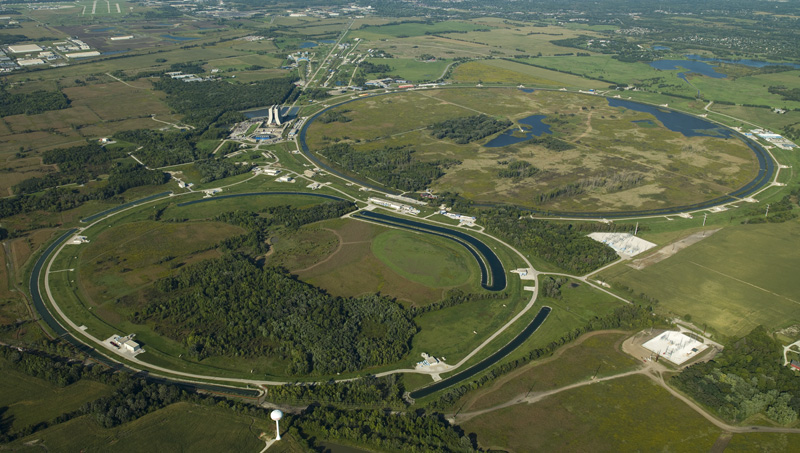
\includegraphics[width=0.7 \linewidth]{Figures/fermilab_facility_07-0329-14D.jpg}
	\end{center}
	\caption{An aerial view of the Fermilab Accelerator complex.
         The Main Injector, from which the protons are extracted onto
         the neutrino target, is in the foreground. (Credit: Fermilab)}
	\label{fig:fermilab_facility_aerial}
\end{figure}


%\subsection{Proton Target, Neutrino Horn, and Decay Volume}

Figure~\ref{fig:numi_horn} shows the layout of the Fermilab NUMI
neutrino production target, focusing horn, decay region (need to
remake the picture with no Minerva and showing 90 degree muons and FWMM). 


\begin{figure}[ht]
	\begin{center}
           	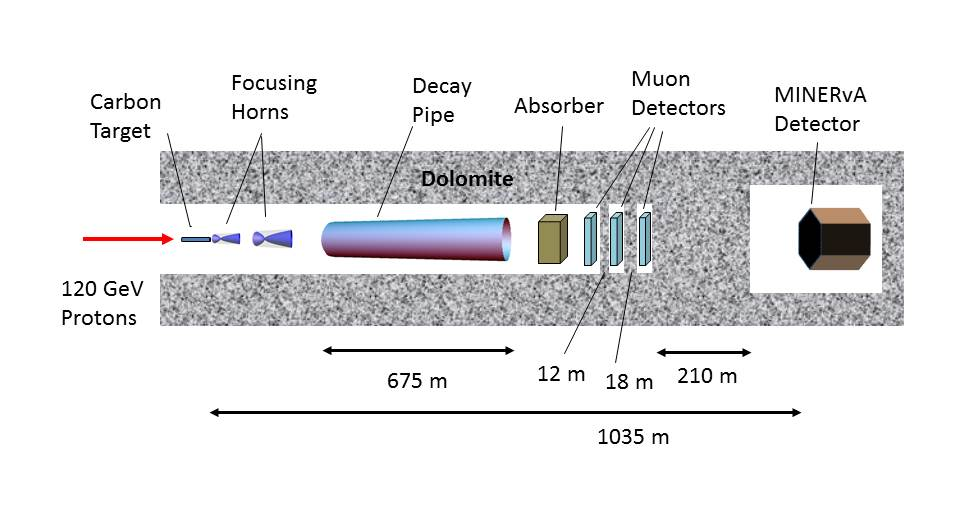
\includegraphics[width=1.0 \linewidth]{Figures/numi_horn_how_works.jpg}
	\end{center}
	\caption{The layout of the Fermilab NUMI neutrino production
          target, focusing horn, decay region, and the Minerva
          experiment. (Credit: Minerva) Needs to be remade no Minerva,
        with TRMM, FWMM}
	\label{fig:numi_horn}
\end{figure}



%\subsection{Properties of the Current Near and Far Detectors}

%\subsection{Constraints: Aperture, the Abort Gap, Radiation Losses, Proton-on-Target}

The proposed superposition of a higher-frequency RF on the current 53
MHz of the Main Injector is subject to several operational
constraints that have impact on the implementation. First, the
aperture of the higher-frequency RF cavity must be large enough not
to limit the MI aperture. Second, during the transition to higher
frequency the longitudinal loss into the abort gap needs to be less
than xxx. Radiation losses from other sources during the transition
must be acceptable. A loss of integrated protons-on-target (POT) due
to the increase in cycle time to accommodate the RF transition should
be small; we take 5\% as a nominal limit. Lastly, cost and schedule
indicate finding an existing hardware solution that can be purchased.

% End of Section 3

